\section{Handwritten digit denoising}
The learn more about the two techniques, both will be applied to a digit recognition problem using the supplied script \texttt{digitsdn}. The original data set consists of handwritten numbers with approximately 20 records per number from $0$ to $9$. Each image has a resolution of $16$ by $15$. Two test sets with one image per numeral are also included. The images are flattened into row vectors and stored in an input matrix with one image The top rows of the plots in figure~\ref{fig:denoise2} show the noise free data of the first test set. The second row noisy versions of the same hand written numbers. 
In the non-linear case the rbf-kernel-function density is initialized using the approximation dimension times the mean of the variance in the training set. Figure~\ref{fig:pcKerLin} shows the principal components found by using linear and kernel pca on the large training data set. These principal components will be used later to clean the noisy numerals in the test set. The plots reveal that a seven shaped principal component is dominant in the kernel as well as the linear case. All rows after the second row in figure~\ref{fig:denoise2} show efforts to reconstruct de-noised versions of the input using an increasing number of principal components. If few components are used the dominant seven shaped vector takes over the reconstruction quite often. If a more complete model with more components is used this does not happen anymore in the linear as well as the nonlinear case. The crucial difference between the two cases is that in the linear case the noise reduction decreases when more principal components are used, resembling the original image more and more. In the kernel case noise reduction gets better each time moving more towards a prototypical representation of the input. This behavior probably stems from the fact that the kernel case is able to adapt better to non-linear number shapes. 
\begin{figure}
\centering
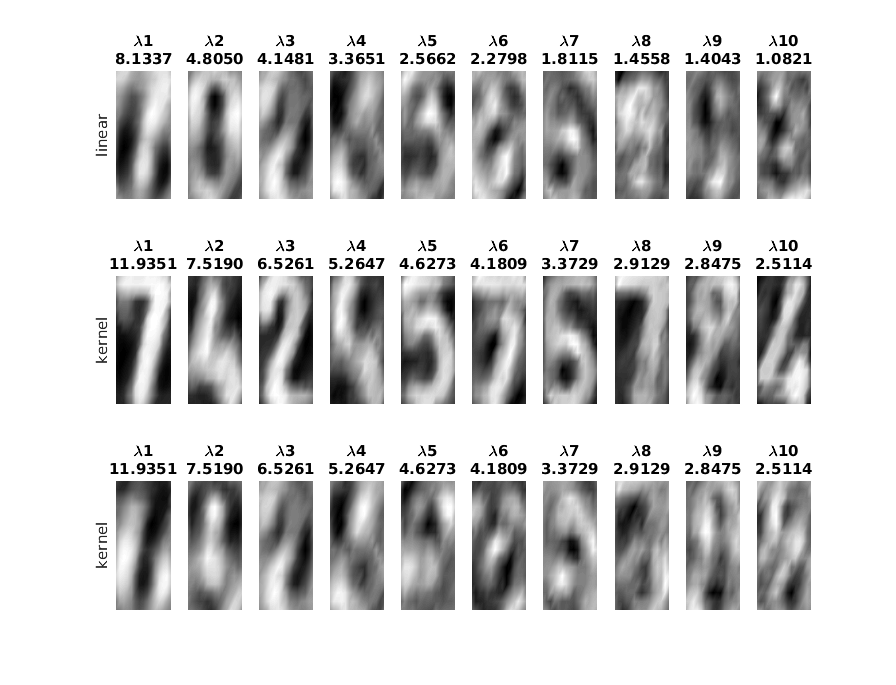
\includegraphics[width=0.7\linewidth]{../src/figure/pcKerLin}
\caption{The principal components using linear PCA (first row). Kernel PCA principal components (second row) and projections using the first principal components (third row).}
\label{fig:pcKerLin}
\end{figure}
\begin{figure}
\centering
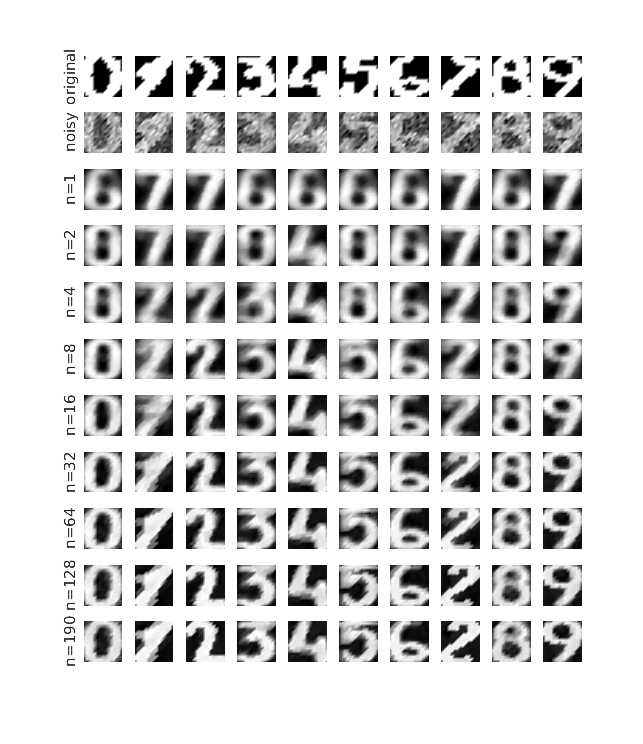
\includegraphics[width=0.49\linewidth]{../src/figure/denoise1}
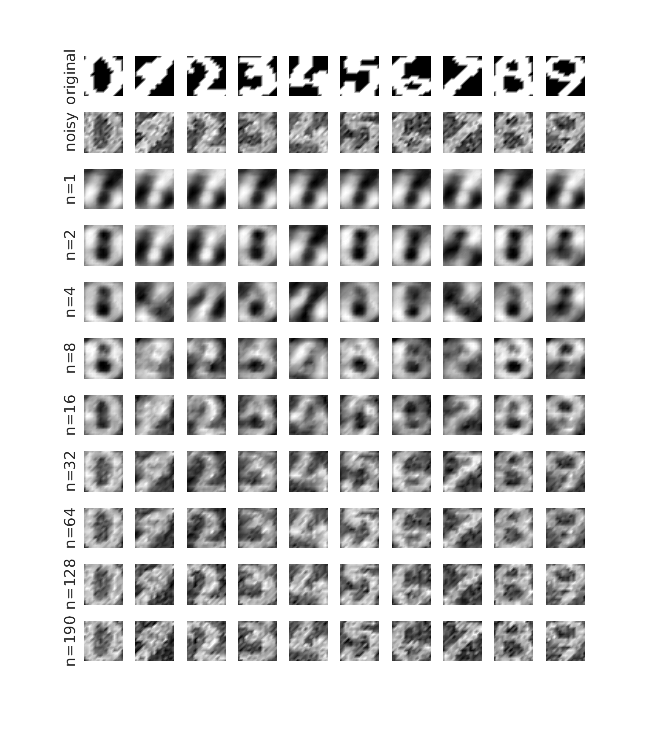
\includegraphics[width=0.49\linewidth]{../src/figure/denoise2}
\caption{Digit de-noising using kernel (left) and linear PCA (right).}
\label{fig:denoise2}
\end{figure}
\begin{figure}
\centering
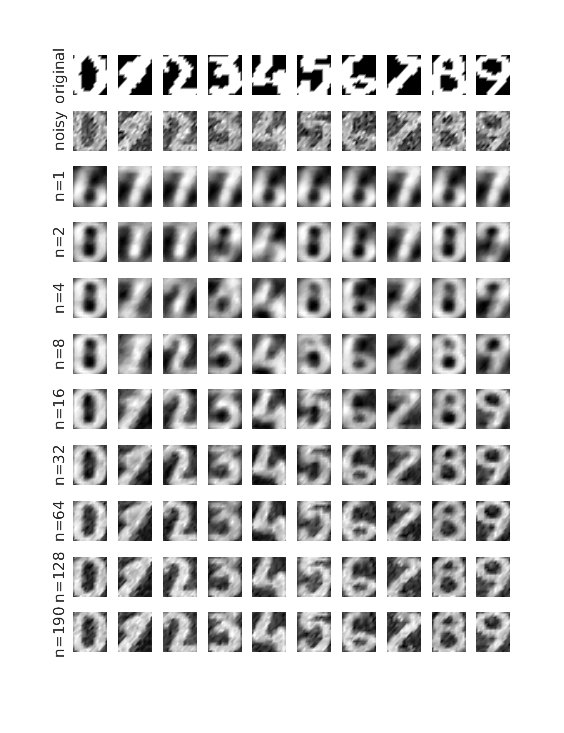
\includegraphics[width=0.49\linewidth]{../src/figure/denoiseKerLargSigm}
\caption{The kernel pca process using an rbf function with larger width $\sigma^2$.}
\label{fig:denoiseKerLargSigm}
\end{figure}
The miss-representation of the number seven in the can be fixed by increasing the rbf-kernel width, the result is shown in figure~\ref{fig:denoiseKerLargSigm}. Unfortunately increasing the width also increases the noise, so a good trade off is required. 



\section{Spectral clustering}